%%%%%%%%%%%%%%%%%%%%%%%%%%%%%%%%%%%%%%%%%%%%%%%%%%%%%%%%%%%%%%%%%%%%%%%%%%%%%%%%
%2345678901234567890123456789012345678901234567890123456789012345678901234567890
%        1         2         3         4         5         6         7         8

\documentclass[letterpaper, 10 pt, conference]{ieeeconf}  % Comment this line out if you need a4paper

%\documentclass[a4paper, 10pt, conference]{ieeeconf}      % Use this line for a4 paper

\IEEEoverridecommandlockouts                              % This command is only needed if 
                                                          % you want to use the \thanks command

\overrideIEEEmargins                                      % Needed to meet printer requirements.

\bibliographystyle{IEEEtran}
\pdfminorversion=4

\usepackage{graphicx}  % Add graphics capabilities
\usepackage{epstopdf} % to include .eps graphics files with pdfLaTeX
 \usepackage{epsfig}
 %\usepackage{psfrag}
 \usepackage{color}
%\usepackage{mathptmx} % assumes new font selection scheme installed
%\usepackage{times} % assumes new font selection scheme installed
\usepackage{amsmath} % assumes amsmath package installed
\usepackage{amssymb}  % assumes amsmath package installed
\usepackage{mathrsfs}
\let\proof\relax
\let\endproof\relax
\usepackage{amsthm}

%\usepackage{graphicx,psfrag,url}

\newtheorem{theorem}{Theorem}
\newtheorem*{remark*}{Remark}
\newtheorem{lemma}{Lemma}
\newtheorem{definition}{Definition}
%\newtheorem{prop}{Proposition}

\DeclareMathOperator*{\argmin}{arg\,min}
\usepackage{bm}
\renewcommand{\qedsymbol}{$\blacksquare$}

\title{Designing Robust Controllers With $H_{\infty}$ Performance Using Frequency-Domain Data}

\author{Achille Nicoletti$^{1}$, and Alireza Karimi$^{1}$
\thanks{$^{1}$A. Nicoletti and A. Karimi are with the Automatic Control Laboratory at Ecole Polytechnique F\'ed\'erale de Lausanne (EPFL), Switzerland.
       Corresponding author: Alireza Karimi: {\tt\small alireza.karimi@epfl.ch}}
\date{September 2015}
}

\begin{document}

\maketitle
\thispagestyle{empty}
\pagestyle{empty}


%%%%%%%%%%%%%%%%%%%%%%%%%%%%%%%%%%%%%%%%%%%%%%%%%%%%%%%%%%%%%%%%%%%%%%%%%%%%%%%%
\begin{abstract}
In this paper, a new frequency-domain method for designing robust controllers is proposed that provides optimal $\mathcal{H}_{\infty}$ performance. A nonlinear optimization problem is formulated which guarantees the stability of the closed-loop system whilst ensuring robust performance. A convexified version of the $\mathcal{H}_{\infty}$ criterion has been established in many works and have utilized a similar frequency gridding process; therefore, it is of interest to determine the definiteness of the solution produced by this convex optimization method with respect to the solution of the optimal $\mathcal{H}_{\infty}$ problem proposed in this work. 
Hello!
\end{abstract}


%%%%%%%%%%%%%%%%%%%%%%%%%%%%%%%%%%%%%%%%%%%%%%%%%%%%%%%%%%%%%%%%%%%%%%%%%%%%%%%%
\section{Introduction}
The uncertainties associated with many of today's complex systems pose challenging tasks for engineers and researchers within the control systems community. These uncertainties can cause performance degradations and stability problems that may lead to catastrophic events. Robust controller design methods seek to rectify this issue by designing controllers that ensure proper stability margins whilst maintaining suitable performance. 

The robust controller design methodology can be realized in two manners: using time-domain or frequency-domain data. In this paper, the frequency-domain approach will be utilized for the controller design scheme. In a data-driven setting, this frequency domain approach can be used to avoid unmodeled dynamics associated with parametric models. A survey on the differences associated with model-based control and data-driven control has been addressed in \cite{HW13} and \cite{BCE12}. The authors in \cite{HDAV10} use the frequency response data of a stable system to design an optimal controller through a symmetric root locus technique. A robust frequency-domain control design method has been established in \cite{KNND13b} that requires a solution to a non-linear optimization problem. A frequency-domain loop-shaping approach to design fixed-structure controllers is presented in \cite{KNND13c}. However, in this method, the closed-loop stability is not guaranteed and should be verified a posteriori.

Robust controller design methods belonging to the $\mathcal{H}_{\infty}$ control framework minimizes the $\mathcal{H}_{\infty}$ norm of a weighted closed-loop sensitivity function. Solving the $\mathcal{H}_{\infty}$ problem can be accomplished in a variety of manners. A convex approximation of the $\mathcal{H}_\infty$ criterion has been discussed in \cite{KG10} and \cite{KGL08} where convex constraints are imposed on the Nyquist diagram. The problem is convexified by constructing a linearly parameterized controller and devising linear constraints with respect to a desired open-loop transfer function.  A frequency-domain approach for computing low-order multivariable linearly parameterized controllers is presented in \cite{SOW10}. The $\mathcal{H}_{\infty}$ constraints are convexified around an initial stabilizing controller. An iterative algorithm is used that converges to a local optimal solution of the non-convex problem. However, in \cite{HAB13},  a convex-concave approximation of the $\mathcal{H}_{\infty}$ constraint is used which is based on an initial stabilizing controller. The extension of this method to design multivariable PID controllers for stable systems is presented in \cite{BHA16}. This method uses the same convex approximation as in  \cite{SOW10} but is limited to stable systems and PID structure. 

In the works asserted above, it has been proved that a convex approximation of the $\mathcal{H}_{\infty}$ problem yields favorable results; however, these approximations do not yield the true global optimal solution to the $\mathcal{H}_{\infty}$ problem. This paper presents an extension of the work in \cite{KNZ16}, and its purpose is to devise a new frequency-domain approach for obtaining the optimal solution to the $\mathcal{H}_{\infty}$ problem. In \cite{KNZ16}, it was shown that the optimal solution is obtained when the order of the controller increases to infinity; in the proposed method, the optimal solution can be obtained for a fixed low-order controller (which has desirable practical implications). A nonlinear optimization problem is formulated to guarantee stability of the closed-loop system while ensuring robust performance (without any approximation). Additionally, it will be shown that the proposed method produces a solution that converges to the global optimal solution of the $\mathcal{H}_{\infty}$ problem under certain conditions. A preset frequency grid will be used to satisfy the robust performance condition and solve for a finite number of constraints. It is desired to compare the solutions produced from the convex optimization algorithms in \cite{KNZ16} with the proposed algorithm and correlate the . 
 
This paper is organized as follows: In Section \ref{sec:pre}, the class of models, controllers and control objectives are defined. Section \ref{sec:problem_form} will address the conditions required for robust performance and the optimization methods used to obtain a solution to the $\mathcal{H}_{\infty}$ problem. Section \ref{sec:sim} will demonstrate the effectiveness of the proposed method and establish the efficacy for the convex approximation of the $\mathcal{H}_{\infty}$ criterion. Finally the concluding remarks are given in Section \ref{sec:conclusion}.

\textbf{Notation}: In order to avoid the risk of any confusion, the notation for the symbols employed in this paper will be defined here. Bolded symbols will represent vectors.
\begin{align*}
\mathbb{R} &: \ \mbox{the set of all real numbers.} \\
\mathbb{R}_+ &: \ \mbox{the set of all real numbers greater than zero.} \\
\Re\{\cdot \} &: \ \mbox{the real part of a complex variable.} \\
\Im\{\cdot \} &: \ \mbox{the imaginary part of a complex variable.} \\
\bm{v} &: \ \mbox{column vector }\bm{v} \mbox{ with elements }[v_1,\ldots,v_n]^{\top}. \\
s &: \ \parbox[t]{18em}{complex frequency variable used to represent continuous-time systems.} \\
z &: \ \parbox[t]{18em}{complex frequency variable used to represent discrete-time systems.}
\end{align*} 

\section{Preliminaries} \label{sec:pre}
\subsection{Class of Models}
The set of all linear time-invariant (LTI) single-input-signal-output (SISO) stable strictly proper models belonging to the family of perturbed plants with multiplicative uncertainty can be defined as follows:
\begin{equation}\label{eq:uncert_set}
\mathcal{G} = \{ G_p(s)[1+\Delta_p(s) W_{2_{p}}(s)]; \quad p=1,\ldots,q\}
\end{equation}  
where $G_p(s)$ is the nominal model of the process, $W_{2_{p}}(s)$ is an uncertainty weight with bounded infinity norm, and $\Delta_p(s)$ is an unknown stable transfer function satisfying $\| \Delta_p \|_{\infty}<1$. For simplicity, one model from the set $\mathcal{G}$ will be analyzed, and the subscript $p$ will be omitted. 

Let the set $\mathscr{P}$ represent the family of all stable, proper, real-rational transfer functions. It is imperative to note that $\mathscr{P}$ is closed under multiplication and addition; in other words, if $P_1(s),P_2(s) \in \mathscr{P}$, then 
\begin{equation}
\{ P_1(s)+P_2(s),P_1(s)P_2(s)\} \in \mathscr{P}
\end{equation}
This definition will also apply to both continuous-time and discrete-time systems. Suppose that a SISO feedback control system structure is used where the plant is represented as $G(s) = N(s)M^{-1}(s)$ such that $\{N(s),M(s)\} \in \mathscr{P}$. As asserted in \cite{ZD98} and \cite{DFT92}, if $\{N(s), M(s)\} \in \mathscr{P}$, then $G(s) = N(s)M^{-1}(s)$ is called a \textit{coprime factorization} of $G(s)$ over $\mathscr{P}$. The controller $K(s) =X(s)Y^{-1}(s)$ can also be described in coprime form, where $\{X(s), Y(s)\} \in \mathscr{P}$.


\subsection{Class of Controllers}
The controllers $X(s)$ and $Y(s)$ for this control scheme will be parameterized in the decision vector $\bm{\rho}$, and can be expressed as
\begin{equation}
\begin{aligned} \label{eq:cont}
X(\bm{\rho},s) &= \bm{\rho}_x^{\top} \bm{\phi}_x(\bm{\rho},s)\\
Y(\bm{\rho},s) &= \bm{\rho}_y^{\top} \bm{\phi}_y(\bm{\rho},s)\\
\end{aligned}
\end{equation}
where $\bm{\rho}_x \in \mathbb{R}^{n_x}$, $\bm{\rho}_y \in \mathbb{R}^{n_y}$, and $\{\bm{\phi}_x(\bm{\rho},s), \bm{\phi}_y(\bm{\rho},s)\}$ are vectors of stable transfer functions chosen from a set of orthogonal basis functions. An example of such a function is the Laguerre basis function \cite{Kar13}:
\begin{equation} \label{eq:Laguerre}
\phi_{\{x,y\}_1}(s)=1,\quad \phi_{\{x,y\}_q}(\bm{\rho},s) = \frac{\sqrt{2 \rho_c}(s-\rho_c)^{q-2}}{(s+\rho_c)^{q-1}}
\end{equation}
for $q = 2,\ldots,n$, where $\rho_c \in \mathbb{R}_+$. For discrete-time systems, the Laguerre basis function can be expressed as follows:
\begin{equation} \label{eq:Laguerre_z}
\phi_{\{x,y\}_1}(z)=1,\quad \phi_{\{x,y\}_q}(\bm{\rho},z) = \frac{\rho_d^*(1-\rho_d z)^{q-2}}{(z-\rho_d)^{q-1}}
\end{equation}
where $\rho_d^* = \sqrt{1-\rho_d^2}$ and $\{\rho_d \in \mathbb{R}: -1 < \rho_d < 1\}$. Note that when $\rho_d = 0$, the discrete-time Laguerre basis function becomes a simple finite-impulse response (FIR) filter.

A PID controller can also be represented in coprime form. Suppose that the desired controller structure is given as:
\begin{equation} \label{eq:pid}
K(\bm{\rho},s)=\rho_1 + \rho_2 \frac{1}{s} + \rho_3 \frac{s}{T_fs+1}
\end{equation}
Then the coprime controllers can be expressed as follows:
\begin{equation}
\begin{aligned} \label{eq:pid_2}
X(\bm{\rho},s) &= \frac{(\rho_1 T_f+\rho_3)s^2 + (\rho_1+\rho_2 T_f)s + \rho_2}{(s+\rho_c^{\prime})^2}\\
Y(\bm{\rho},s) &= \frac{s(T_fs+1)}{(s+\rho_c^{\prime})^2}
\end{aligned}
\end{equation}
where $\rho_c^{\prime} \in \mathbb{R}_+$. With the PID, note that if $\rho_c^{\prime}$ is fixed, then the coprime $X$ is linearly parameterized while $Y$ is a TF independent of the decision variables. This will always be the case when the controller $K$ is linearly parameterized.
\section{Problem Formulation} \label{sec:problem_form}
The methods described in this paper are associated with minimizing the $\mathcal{H}_{\infty}$ norm of a desired weighted sensitivity function. The sensitivity function $S(s)$ and complementary sensitivity function $T(s)$ associated with this control scheme can be formulated as follows:
\begin{equation}
\begin{aligned} \label{eq:S}
S(s) &:= e/r =[1+L(\bm{\rho},s)]^{-1} \\ &=  M(s)Y(\bm{\rho},s)[N(s)X(\bm{\rho},s)+M(s)Y(\bm{\rho},s)]^{-1}\\
\end{aligned}
\end{equation}
\begin{equation}
\begin{aligned} \label{eq:T}
T(s) &:= y/r =L(\bm{\rho},s)[1+L(\bm{\rho},s)]^{-1} \\ &=  N(s)X(\bm{\rho},s)[N(s)X(\bm{\rho},s)+M(s)Y(\bm{\rho},s)]^{-1}\\
\end{aligned}
\end{equation}
where $L(s) = G(s)K(s)$; $r$ is the reference input; $y$ is the system output; $e$ is the tracking error signal (i.e., $e = r-y$). From the above definitions of the sensitivity functions, it can be observed that $S(s)+T(s)=1$.

\subsection{Robust Performance via Convex Optimization}
Consider a process from the multiplicative uncertainty set in (\ref{eq:uncert_set}). Given a performance weighting filter $W_1(s)$ with bounded infinity norm, a necessary and sufficient condition for achieving robust performance is given by \cite{DFT92}:
\begin{equation}\label{eq:inf_norm}
\| |W_1 S| + |W_2 T| \|_{\infty} < \gamma
\end{equation}
where $\gamma = 1$. However, the problem of minimizing the upper bound $\gamma$ will be considered in this paper, where $ \gamma \in \mathbb{R}_+$. The condition in (\ref{eq:inf_norm}) can also be expressed as
\begin{equation} \label{eq:inf_norm2}
|W_1(j\omega)S(\bm{\rho},j\omega)|+|W_2(j\omega)T(\bm{\rho},j\omega)|<\gamma, \quad \forall \omega \in \Omega
\end{equation}
where $\Omega \in [0,\infty)$. For notation purposes, the dependence in $j\omega$ will be omitted and will only be reiterated when deemed necessary. The dependence on $\bm{\rho}$ will continue to be highlighted. By substituting (\ref{eq:S}) and (\ref{eq:T}) into (\ref{eq:inf_norm2}), the condition for robust performance can be expressed as
\begin{equation} \label{eq:circle}
\gamma^{-1}\left[ |W_1MY(\bm{\rho})| + |W_2 NX(\bm{\rho})| \right] < |\psi(\bm{\rho})|, \quad \forall \omega \in \Omega
\end{equation}

\begin{figure}
\centering
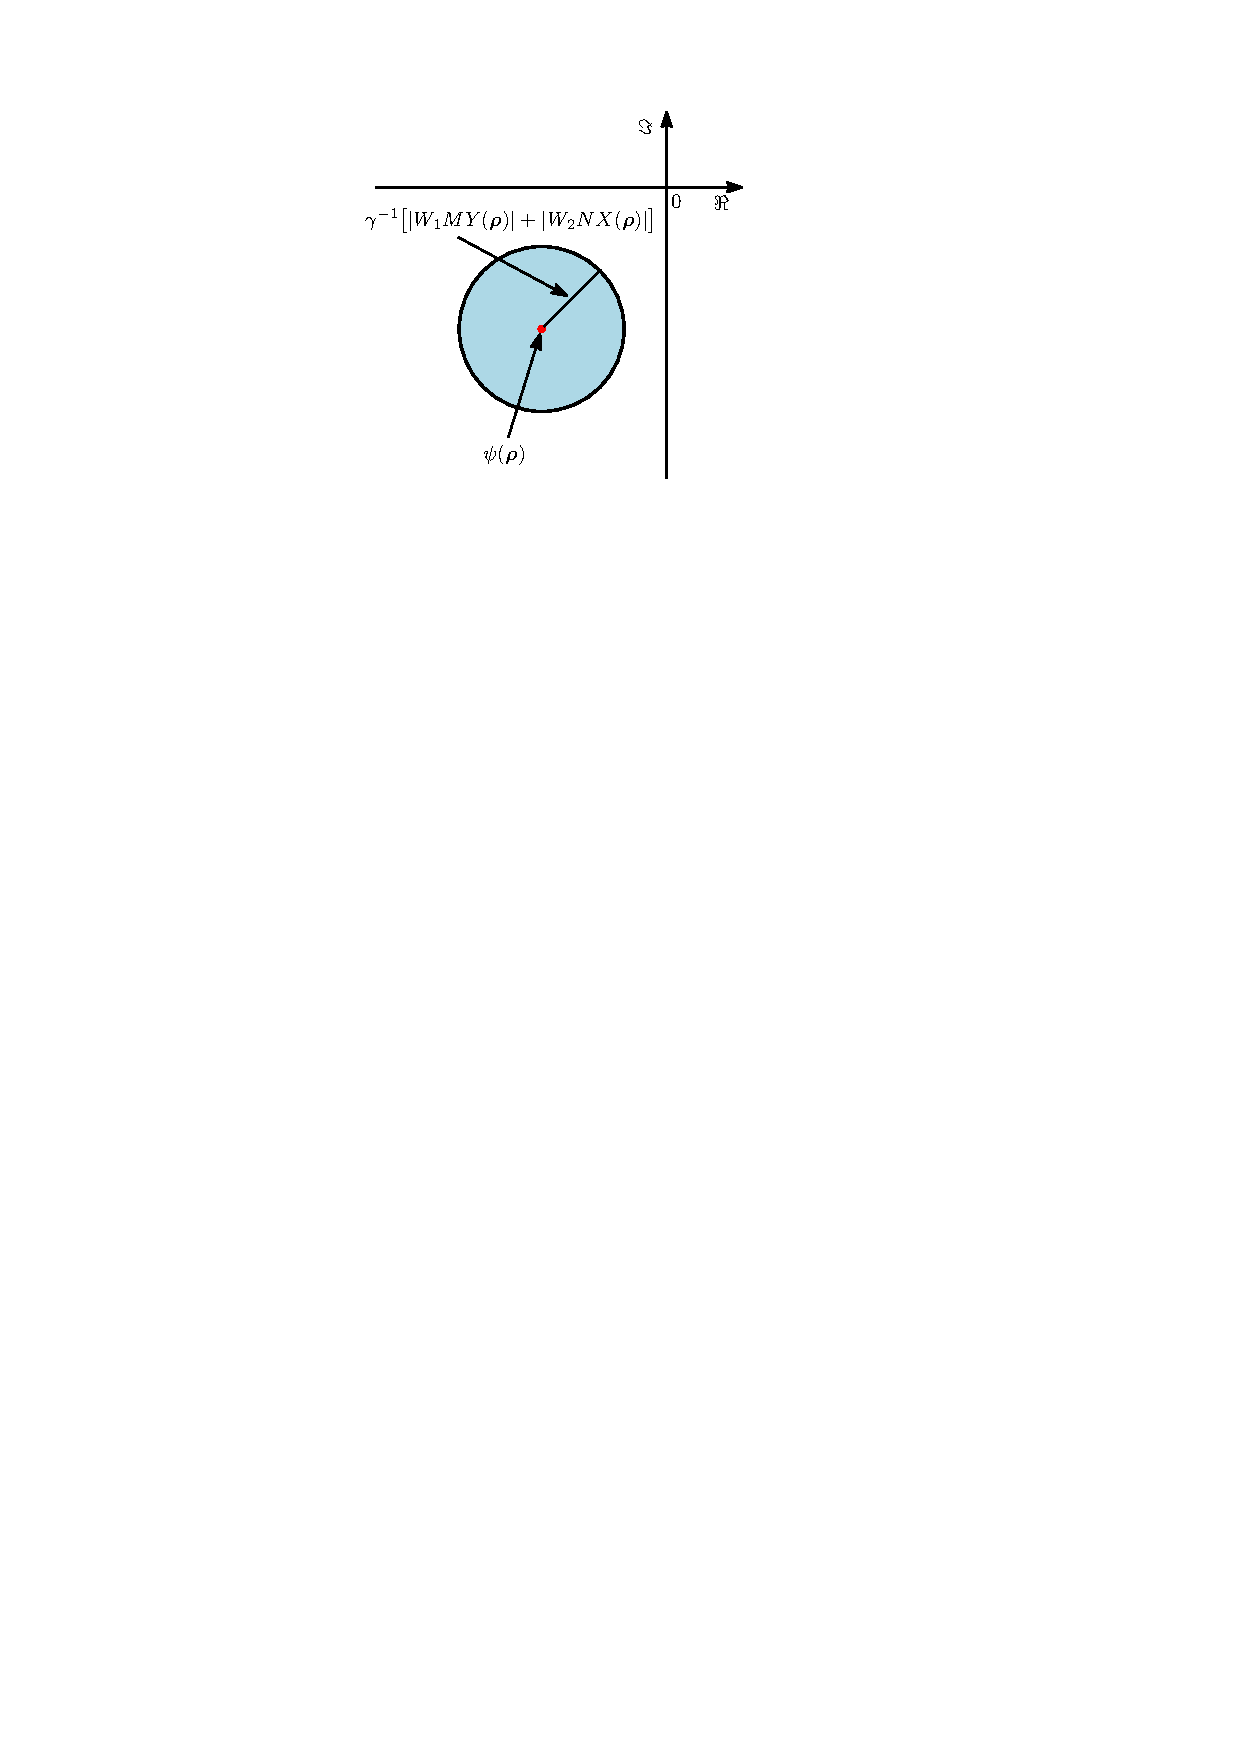
\includegraphics[width=0.7\columnwidth]{../pics/circle_rotation_RP.pdf}
\caption{Graphical interpretation of the $\mathcal{H}_\infty$ robust performance constraint in the complex plane.}
\label{fig:circle}
\end{figure}

where $\psi(\bm{\rho}) = NX(\bm{\rho})+MY(\bm{\rho})$. Consider a circle in the complex plane at a specific frequency in $\Omega$ which is centered at $\psi(\bm{\rho})$ and has radius $\gamma^{-1}\left[ |W_1MY(\bm{\rho})| + |W_2 NX(\bm{\rho})| \right]$ (as shown in Fig.~\ref{fig:circle}). The constraint in (\ref{eq:circle}) ensures that for any frequency point in $\Omega$, the circle associated with this frequency point will not encircle the origin. In \cite{KNZ16}, the authors show that there exists a function $F(s)$ that can rotate this circle such that it lies on the right-hand side of the $j\omega$ axis of the complex plane (i.e., all values on and within the circle have positive real parts). This condition is recalled with the following Lemma:

\begin{lemma}   \label{lem1}
Suppose that 
\begin{equation*}
\begin{aligned}
H_1(\bm{\rho}) &=W_1MY(\bm{\rho}) \psi^{-1}(\bm{\rho})\\   H_2(\bm{\rho}) &=W_2NX(\bm{\rho}) \psi^{-1}(\bm{\rho})
\end{aligned}
\end{equation*}
are frequency responses of bounded analytic functions in the right-half plane. Then, the following constraint is met
\begin{equation} \label{eq4}
\sup_{\omega \in \Omega}  \big(|H_1(\bm{\rho}) | + |H_2(\bm{\rho}) | \big) < \gamma
\end{equation}
if and only if there exists a stable transfer function $F(s)$ that satisfies
$$
\Re\{\psi(\bm{\rho})F\}>\gamma^{-1}\left[ |W_1MY(\bm{\rho})F| + |W_2 NX(\bm{\rho})F| \right]
$$
for all $\omega \in \Omega $
\end{lemma}
{\it Proof :} 
The proof of a similar condition has been formally documented in \cite{KNZ16}. Here, the condition has been extended for attaining robust performance instead of nominal performance.
{\hfill \ensuremath{\blacksquare}}

With the above Lemma, a necessary and sufficient condition can be derived for attaining robust performance. In \cite{KNZ16}, it is shown that if $X(\bm{\rho})$ and $Y(\bm{\rho})$ are linearly parameterized, then a convex optimization problem can be formulated as follows: 
\begin{equation} \label{eq:convex_con}
\begin{aligned}
& \underset{ \bm{\rho}}{\text{minimize}}
& & \gamma  \\
& \text{subject to:} & & \gamma^{-1} \left[  |W_1MY(\bm{\rho})| + |W_2 NX(\bm{\rho})| \right] < \Re\{\psi(\bm{\rho}) \}  \\ 
& & & \forall \omega \in \Omega \quad 
\end{aligned}
\end{equation}
Notice that (\ref{eq:convex_con}) is a semi-infinite programming (SIP) optimization problem since there are a finite number of optimization variables and an infinite number of constraints. This problem can be solved by presetting a frequency grid $\omega$ and solving a finite number of constraints. This frequency grid can be predefined in a variety of manners (see \cite{SVBB11}, \cite{GKL10b}).

\subsection{Optimal Performance via Nonlinear Programming}
In \cite{KNZ16}, it is shown that when the orders of $X(\bm{\rho})$ and $Y(\bm{\rho})$ approach infinity, then $\gamma$ from (\ref{eq:convex_con}) approaches the optimal solution to the $\mathcal{H}_{\infty}$ problem. However, it is impractical and sometimes impossible to implement large order controllers in a real system.

One solution to this problem is to find the optimal solution for a fixed low-order controller. According to Lemma \ref{lem1}, it is known that there exists a stable transfer function $F$ such that the constraint to the $\mathcal{H}_{\infty}$ problem is satisfied. Therefore, the optimal solution to this problem can be accomplished by fixing the orders of $X(\bm{\rho})$ and $Y(\bm{\rho})$ and implementing the following optimization problem:
\begin{equation} \label{eq:opt_true}
\begin{aligned}
& \underset{ \bm{\rho}}{\text{minimize}}
& & \gamma  \\
& \text{subject to:} & & \gamma^{-1} |F(\bm{\rho})|\big[  |W_1MY(\bm{\rho})| + |W_2 NX(\bm{\rho})| \big] \\ &&& \hspace{3.3cm}<   \Re\{F(\bm{\rho})\psi(\bm{\rho}) \}  \\ 
& & & \forall \omega \in \Omega \quad 
\end{aligned}
\end{equation}
where $F(\bm{\rho})$ can be chosen such that it incorporates the Laguerre basis functions defined in (\ref{eq:Laguerre}), i.e.,
\begin{equation} \label{eq:Laguerre_sum_c}
F(\bm{\rho}) = \rho_{f_{1}}+ \sum_{p=2}^{q} \rho_{f_{p}}\frac{\sqrt{2 \rho_o}(s-\rho_o)^{p-2}}{(s+\rho_o)^{p-1}}
\end{equation}
where $\rho_o \in \mathbb{R}_+$. It will now be shown that the solution to the optimization problem in (\ref{eq:opt_true}) converges to the optimal solution of the $\mathcal{H}_\infty$ problem as the order of $F(\bm{\rho})$ increases. The proof will omit the dependence on $\bm{\rho}$ since the result is independent on the parameterization of the basis functions.

\begin{theorem} \label{thm_1}
Suppose that the controller $K_o(s)$ achieves the optimal $\mathcal{H}_\infty$ robust performance condition for the plant model $G(s) = N(s)M^{-1}(s)$ such that
\begin{equation}
\gamma_o = \sup_{\omega \in \Omega} \bigg(  \left|W_1(1+L_o)^{-1}\right|  + \left|W_2L_o(1+L_o)^{-1}\right|  \bigg)
\end{equation}
where $L_o = GK_o$. Additionally, suppose that $\gamma_n$ is the optimal solution of the problem in (\ref{eq:opt_true}) when $X$ and $Y$ are constructed such that $K = XY^{-1}$ has the same structure as $K_o$ and $F$ is parameterized by an $n$ dimensional orthogonal basis function. Then $\gamma_n$ converges monotonically from above to $\gamma_o$ when $n \rightarrow \infty$.
\end{theorem}
{\it Proof :} 
According to Lemma.\ref{lem1}, there exists $\{X_o(s),Y_o(s)\} \in \mathscr{P}$ and stable transfer function $F_o(s)$ such that $K_o(s) = X_o(s)Y_o^{-1}(s)$ and
\begin{equation}\label{eq:the_eq_1}
\gamma_o = \sup_{\omega \in \Omega} \bigg(  \left|\frac{W_1MY_oF_o}{\Re \{ \psi_oF_o\}} \right| +\left|\frac{W_2NX_oF_o}{\Re \{ \psi_oF_o\}} \right| \bigg)
\end{equation}
where $\psi_o = NX_o+MY_o$. Now take $F_n^*$ as the projection of $F_o$ into the subspace spanned by an $n$ dimensional orthogonal basis function and define the following quantity:
\begin{equation} \label{eq:the_eq_2}
\gamma_n^* = \sup_{\omega \in \Omega} \bigg(  \left|\frac{W_1MY_oF_n^*}{\Re \{ \psi_oF_n^*\}} \right| +\left|\frac{W_2NX_oF_n^*}{\Re \{ \psi_oF_n^*\}} \right| \bigg)
\end{equation}
By contradiction, is can be shown that $\gamma_n^*$ is a bounded function (using the fact that $\Re \{ \psi_oF_o\} > \epsilon > 0$); assume that $j\omega^*$ is a zero of $\Re \{ \psi_o F_n^*\}$. Therefore, at $\omega=\omega^*$,
\begin{equation}
\Re \{ \psi_oF_o\}  = \Re \{ \psi_o(F_o-F_n^*)\} > \epsilon
\end{equation}
However, $\Re \{ \psi_o(F_o-F_n^*)\}$ can be made arbitrarily small by increasing $n$; therefore, for a large but finite $n$, $\Re \{ \psi_o F_n^*\} \neq 0$.

By using the relations in (\ref{eq:the_eq_1}) and (\ref{eq:the_eq_2}), one can compute $|\gamma_o - \gamma_n^*|$ as follows:
\begin{equation}
\begin{split}
|\gamma_o - \gamma_n^*|  & \leq \sup_{\omega \in \Omega} \bigg| \frac{|W_1MY_oF_o| + |W_2NX_oF_o|}{|\Re \{\psi_o F_o \}|}  \\  & \hspace{2cm}- \frac{|W_1MY_oF_n^*| + |W_2NX_oF_n^*|}{| \Re \{\psi_o F_n^* \}|} \bigg|
\end{split}
\end{equation}
However, according to \cite{AN99b}, it is known that
\begin{equation}
\lim_{n \to \infty} \|F_o - F_n^* \|_{\infty} = 0
\end{equation}
From this relation, it can be deduced that $\lim_{n \to \infty} |F_n^*| \rightarrow |F_o|$ and $\lim_{n \to \infty} \Re \{F_n^*\} \rightarrow \Re\{F_o\}$. Therefore, we obtain the following result:
\begin{equation}
\lim_{n \to \infty} |\gamma_o - \gamma_n^*|  = 0
\end{equation}
However, $\gamma_n$ (the solution to the optimization problem in (\ref{eq:opt_true})) is always less than or equal to $\gamma_n^*$ and greater that the optimal solution $\gamma_o$ if the structures of $X$ and $Y$ are the same as $X_o$ and $Y_o$, respectively. Therefore, $\gamma_n$ converges from above to $\gamma_o$, and this convergence is monotonic because the basis functions $F_n$ of order $n$ are a subset of those of order $n+1$, which ensures that $\gamma_{n+1} \leq \gamma_n$.
{\hfill \ensuremath{\blacksquare}}

Note that the constraint in the optimization problem (\ref{eq:opt_true}) is not convex and a non-linear optimization algorithm will need to be implemented in order to solve this problem. In this manner, the parameter $\rho_o$ in $F(\bm{\rho})$ need not be fixed, and the optimal solution can be obtained for a lower-order $F(\bm{\rho})$ (as will be demonstrated in subsequent sections of this paper).

\begin{remark*}
One problem with solving the nonlinear problem in (\ref{eq:opt_true}) is defining the initial conditions. Since there can be many variables involved in this optimization problem, defining the initial conditions to achieve the global optimal solution to the $\mathcal{H}_{\infty}$ problem may not be trivial. One solution to this problem is to first solve the convex optimization problem in (\ref{eq:convex_con}) and use the solution to this problem as the initial conditions for the nonlinear problem in (\ref{eq:opt_true}). In this manner, the likelihood of obtaining the global optimal solution to the nonlinear problem will significantly increase. 
\end{remark*}

\iffalse
PSO is a powerful optimization method that can solve both linear and nonlinear problems. It is based on the principle that groups of individuals work together to improve both their collective and individual performance \cite{Sim13}. Due to the constraints imposed in (\ref{eq:opt_true}), an exterior method (i.e., Non-Death-Penalty approach) will be implemented in order to obtain the optimal solution to the problem. With this method, the constrained optimization problem can be transformed to the following unconstrained problem:
\begin{equation} \label{eq:pso_obj}
\underset{ \{ \bm{\rho}\in \mathbb{R}^n,\gamma \in \mathbb{R}\}}{\text{minimize}} \ \ \Phi(\bm{\rho},\gamma)
\end{equation}
where
\begin{equation} \label{eq:pso_hinf}
\begin{aligned}
\Phi(\bm{\rho},\gamma) &= \gamma + \frac{1}{N}\sum_{k=1}^N \alpha_k Z_k(\bm{\rho},\gamma) \\
Z_k(\bm{\rho},\gamma) &= [\mbox{max}(0,z_k(\bm{\rho},\gamma))]^\beta \\
z_k(\bm{\rho},\gamma) &=   |W_1(j\omega_k)M(j\omega_k)Y(\bm{\rho},j\omega_k)F(\bm{\rho},j\omega_k)| \\ & \hspace{1cm}+ |W_2(j\omega_k) N(j\omega_k)X(\bm{\rho},j\omega_k)F(\bm{\rho},j\omega_k)|  \\ &\hspace{3cm} -  \gamma \Re\{F(\bm{\rho},j\omega_k)\psi(\bm{\rho},j\omega_k) \}  
\end{aligned}
\end{equation}
The value of $\beta$ is usually taken to be $1$ or $2$ and $\alpha_k \in \mathbb{R}$ is the penalty factor \cite{Sim13} . In this paper, $\beta=1$ will be considered. For this particular problem, the value of $\alpha_k$ will be a constant, since the weighting factor for each constraint should be the same ($\alpha_k=\alpha$). In other words, the constraint should not be weighted differently for varying frequencies. Since $\gamma \geq 1$, the value of $\alpha$ should be chosen such that $\psi(\bm{\rho},\gamma) \gg 1$ for all particles in the initialized population. 

The PSO algorithm seeks to find an optimal solution by implementing a swarm of $m_p$ particles. Let $\bm{x}_i$ denote the position of the $i^{th}$ particle; for the decision variables considered in (\ref{eq:pso_hinf}), the $i^{th}$ particle occupies the position\footnote{Note that $\gamma_i$ in this context represents the position of the $i^{th}$ particle, and not the $i^{th}$ iteration of the bisection algorithm asserted in the remark in the previous section.}
\begin{equation}
\bm{x}_i := [\rho_{i,1},\rho_{i,2},\ldots,\rho_{i,n},\gamma_i]^{\top} \in \mathbb{R}^{n+1} 
\end{equation}
where $i \in \{1,\ldots,m_p \}$. The velocity of the $i^{th}$ particle (at which it moves though the search space) is denoted as
\begin{equation}
\bm{v}_i := [v_{i,1},v_{i,2},\ldots,v_{i,n},v_{i,\gamma}]^{\top} \in \mathbb{R}^{n+1}. 
\end{equation}
One approach in expressing the manner in which the position and velocity of the $i^{th}$ particle is updated can be realized as
\begin{equation} \label{eq:update}
\begin{aligned}
\bm{x}_i^{l+1} &= \bm{x}_i^{l} + \bm{v}_i^{l+1} \\
\bm{v}_i^{l+1} &= K [ \bm{v}_i^l + \theta_1 r_{1,i}^l(\bm{b}_i^l-\bm{x}_i^l) + \theta_2 r_{2,i}^l(\bm{h}_i^l-\bm{x}_i^l) \\
& \hspace{3.7cm}+ \theta_3 r_{3,i}^l(\bm{g}^l-\bm{x}_i^l) ]
\end{aligned}
\end{equation}
where $K \in \mathbb{R}$ is the constriction coefficient, and $\theta_c \in \mathbb{R}$ for $c \in \{1,2,3 \}$ are the learning rates ($\theta_1$ is the cognitive learning rate, $\theta_2$ is the social learning rate, and $\theta_3$ is the learning rate influencing the best individual found so far since the first generation). The random numbers $r_{c,i}^l$ are uniformly distributed in $[0, 1]$ and represent the stochastic behavior associated with the algorithm. For a stable PSO algorithm, the constriction coefficient should be chosen as follows \cite{Sim13}: 
\begin{equation}
K = \frac{2 k_\alpha}{\theta_T-2}
\end{equation}
where $k_\alpha \in (0,1)$ and $\theta_T = \theta_1 + \theta_2 +\theta_3$. The best-so-far position of the $i^{th}$ particle is defined as
\begin{equation}
\bm{b}_i^l = \argmin_{ \bm{x}_i^t} \{\Phi(\bm{x}_i^t),0\leq t \leq l \}.
\end{equation}
For a given neighborhood size $\sigma$, the best-so-far position of $\sigma$ close neighbors is determined as follows:
\begin{equation}
\bm{h}_i^l = \argmin_{\bm{x}_i^t} \{\Phi(\bm{x}_i^t),0\leq t \leq l\mid \bm{x}_i^t \in H_i^t \}
\end{equation}
where $H_i^t$ are the $\sigma$ nearest neighbors of $\bm{x}_i^t$. The best position of the entire swarm for the current iteration $l$ is defined as
\begin{equation}
\bm{g}^l = \argmin_{\bm{x}_i^l} \{\Phi(\bm{x}_i^l), \forall i \}.
\end{equation}
The PSO algorithm can be summarized with the following steps:

\begin{enumerate}
  \def\makelabel{Step~}
  \item{Initialize a population of $m_p$ particles with random positions $\bm{x}_i^0 \ \forall i$ and velocities $\bm{v}_i^0=0$. Evaluate $\psi(\bm{x}_i^0)$. For a given value of $\alpha_k$ in (\ref{eq:pso_hinf}), ensure that $\psi(\bm{x}_i^0) \gg 1$ for every particle in the population. If $\psi(\bm{x}_i^0) < 1 \ \forall i$, increase the value of $\alpha_k$. Set $l=0$ and determine $\bm{b}_i^0$, $\bm{h}_i^0$, and $\bm{g}^0$.}
  \item{Apply the update equations in (\ref{eq:update}) and evaluate the cost function with the new population. }
  \item{If the termination criterion is satisfied, then the algorithm returns the optimal solution 
  \begin{equation}
  \bm{x}^{\star} = \argmin_{\bm{x}_i^k} \{\psi(\bm{x}_i^k), \forall i,k \}.
  \end{equation} Otherwise, go to the next step.}
  \item{Set $l=l+1$ and determine $\bm{b}_i^l$, $\bm{h}_i^l$, and $\bm{g}^l$. Then return to Step $2$.}
\end{enumerate}
The optimal values of $\theta_c$ may vary depending on the problem that is being analyzed; in general, it is recommended that $\theta_c=2.1 \ \forall c$ \cite{Sim13}. A similar rationalization can be made with the selection of $k_\alpha$; a larger value of $k_\alpha$ encourages exploration while a smaller value of $k_\alpha$ bolsters exploitation. 
 \fi

\section{Simulation Examples} \label{sec:sim}
Let us now consider several examples in order to determine the validity of the proposed method. For each example, the \texttt{MATLAB} software was used in conjunction with the \texttt{fmincon} function to solve the proposed optimization problem. 

\subsection{Example 1: Robust Performance}
Consider the unstable non-minimum phase system analyzed in \cite{Zhe10}  and \cite{Ho03} (which is subject to multiplicative uncertainty):
\begin{equation}
G(s) = \frac{s-1}{s^2+0.8s-0.2}
\end{equation}
The objective of this case study is to design a stabilizing PID controller such that the robust performance condition in (\ref{eq:inf_norm}) is satisfied. The weighting filters for this design will be chosen as those defined in \cite{Zhe10}:
\begin{equation}
W_1(s) = \frac{10}{100s+1}, \quad W_2(s) = \frac{s+0.1}{s+1}
\end{equation}
Since $G(s)$ is unstable, the coprime functions can be selected as follows:
\begin{equation}
N(\bm{\rho},s) = \frac{s-1}{(s+\rho_g)^2}, \quad M(\bm{\rho},s) = \frac{(s^2+0.8s-0.2)}{(s+\rho_g)^2}
\end{equation}
where $\rho_g \in \mathbb{R}_+$. For a PID controller, the structure of the controllers $X(\bm{\rho})$ and $Y(\bm{\rho})$ can be selected as those defined in (\ref{eq:pid_2}) with $T_f = 0.01$. 
\subsubsection{Simulation Results}
The problem in (\ref{eq:opt_true}) is solved by converting it to an SDP problem and gridding the frequency from $10^{-3}$ to $10^{3} \ rad/s$ (using $500$ logarithmically spaced points). A $20$-th order basis function for $F(\bm{\rho})$ is selected (as defined in (\ref{eq:Laguerre_sum_c})). For comparative purposes, the \texttt{MATLAB} \texttt{mixsyn} function from the Robust Control Toolbox is used to compute a controller with the given weighting filters; the toolbox yields a $4$-th order controller. 

Table.\ref{tab:ex1_1} shows the values of the optimal solutions obtained from various methods. The convex problem in (\ref{eq:convex_con}) was solved with $\rho_g = \rho_c^{\prime} = 1$. Since \texttt{mixsyn} minimizes $\|[W_1S \ \ W_2T] \|_\infty$, it can be observed that a smaller value of this criteria is obtained (with a $4$-th order controller). However, with a simple PID controller, the proposed method yields the best performance for the \textit{true} robust performance criteria in (\ref{eq:inf_norm}). The optimal value for the the decision variable of $F(\bm{\rho})$ was obtained as $\rho_o^{\star} = 0.933$, while the optimal values of the remaining decision variables (for both the convex and proposed optimization methods) are shown in Table.\ref{tab:ex1_2}. 

\begin{table}[]
\centering
\caption{My caption}
\label{tab:ex1_1}
\begin{tabular}{c|c|c}
                                                                                                          & $\| |W_1S| + |W_2T| \|_{\infty}$ & $\left\| \begin{matrix} W_1S \\[2pt] W_2T \end{matrix} \right\|_{\infty} $ \\ \hline
\texttt{MATLAB\textsuperscript{\tiny{\textregistered}}} (\texttt{mixsyn})                                                                           & $1.111$                          & $0.789$                                                     \\ \hline
\begin{tabular}[c]{@{}c@{}}$\mathcal{H}_\infty$ parametric\\ approach in \cite{Kar13}\end{tabular}                                                                                     & $1.205$                          & $0.923$                                                     \\ \hline
\begin{tabular}[c]{@{}c@{}}Proposed method\end{tabular}  & $1.019$                          & $0.966$ \\ \hline                                                                                                 
\begin{tabular}[c]{@{}c@{}}Convex method (\ref{eq:convex_con})\end{tabular}  & $1.327$                          & $1.223$
\end{tabular}
\end{table}

\begin{table}[]
\centering
\caption{My caption}
\label{tab:ex1_2}
\begin{tabular}{c|c|cccc}
                                                          & $\rho_1^{\star}$ & $\rho_2^{\star}$              & $\rho_3^{\star}$              & $\rho_g^{\star}$             & $(\rho_c^{\prime})^{\star}$ \\ \hline
\begin{tabular}[c]{@{}c@{}}Convex\\ Method (\ref{eq:convex_con})\end{tabular}   & $-0.565$         & \multicolumn{1}{c|}{$-0.013$} & \multicolumn{1}{c|}{$-0.397$} & \multicolumn{1}{c|}{$1$}     & $1$                         \\ \hline
\begin{tabular}[c]{@{}c@{}}Proposed\\ Method (\ref{eq:opt_true})\end{tabular} & $-0.486$         & \multicolumn{1}{c|}{$-0.021$} & \multicolumn{1}{c|}{$-0.486$} & \multicolumn{1}{c|}{$1.647$} & $1.647$                    
\end{tabular}
\end{table}

\subsection{Example 2: Convergence to Optimal Solution}
Consider the following discrete time SISO system:
\begin{equation}
G(z) = \frac{z-0.186}{z^3 - 1.116z^2 + 0.465z-0.093}
\end{equation}
Note that since this system is stable, then the coprimes can be selected as $N(z) = G(z)$ and $M(z) = 1$. The control objective of this case study is to design a controller (with integral action) that minimizes the nominal performance condition $\|W_1S \|_{\infty}$ (i.e., minimize $\gamma$ in $\|W_1S \|_{\infty} < \gamma$), where
\begin{equation}
W_1(z) = \frac{0.4902(z^2-1.0431z+0.3263)}{(z-1)(z-0.282)}
\end{equation}
For this controller synthesis, we can simply select the basis functions in (\ref{eq:Laguerre_z}) to be FIR filters (i.e., $\rho_d = 0$) for $X(\bm{\rho})$ and $Y(\bm{\rho})$. In order to avoid unboundedness of $W_1$ at $\omega = 0$ and have integral action, the basis functions for $Y(\bm{\rho})$ will be multiplied by $(z-1)/z$. It will be shown that as the order of $F(\bm{\rho})$ increases, the optimal solution $\gamma$ will decrease monotonically and converge to the optimal solution. 

\subsubsection{Simulation Results}
The \texttt{mixsyn} command from \texttt{MATLAB}'s Robust Control toolbox yields an optimal value of $\gamma^* = 0.5522$ with a fifth-order controller. Therefore, according to Theorem.\ref{thm_1}, a fifth-order controller was also implemented with the proposed method (i.e., to ensure convergence to the optimal solution). Additionally, two simulations were performed with the proposed method; one simulation with $F(\bm{\rho})$ selected such that the basis function is an FIR filter (i.e., Laguerre basis functions in (\ref{eq:Laguerre_z}) with $\rho_d = 0$) and one simulation with $F(\bm{\rho})$ selected such that $\rho_d$ is a decision variable.  Let $F_{n_f}(\bm{\rho})$ denote the function $F(\bm{\rho})$ of $n_f$-th order and $\gamma_{n_f}$ denote the optimal solution of the nominal performance condition for a given order of $F_{n_f}(\bm{\rho})$. Figure.~\ref{fig:ex2} shows the convergence of the optimal solution $\gamma_{n_f}$ as a function $n_f$; it can be observed that with the proposed frequency-domain method, the optimal solution to the $\mathcal{H}_{\infty}$ problem converges monotonically as the order of $F(\bm{\rho})$ increases. Additionally, when the parameter $\rho_d$ is a decision variable, the convergence time is reduced. 

\begin{figure}
\centering
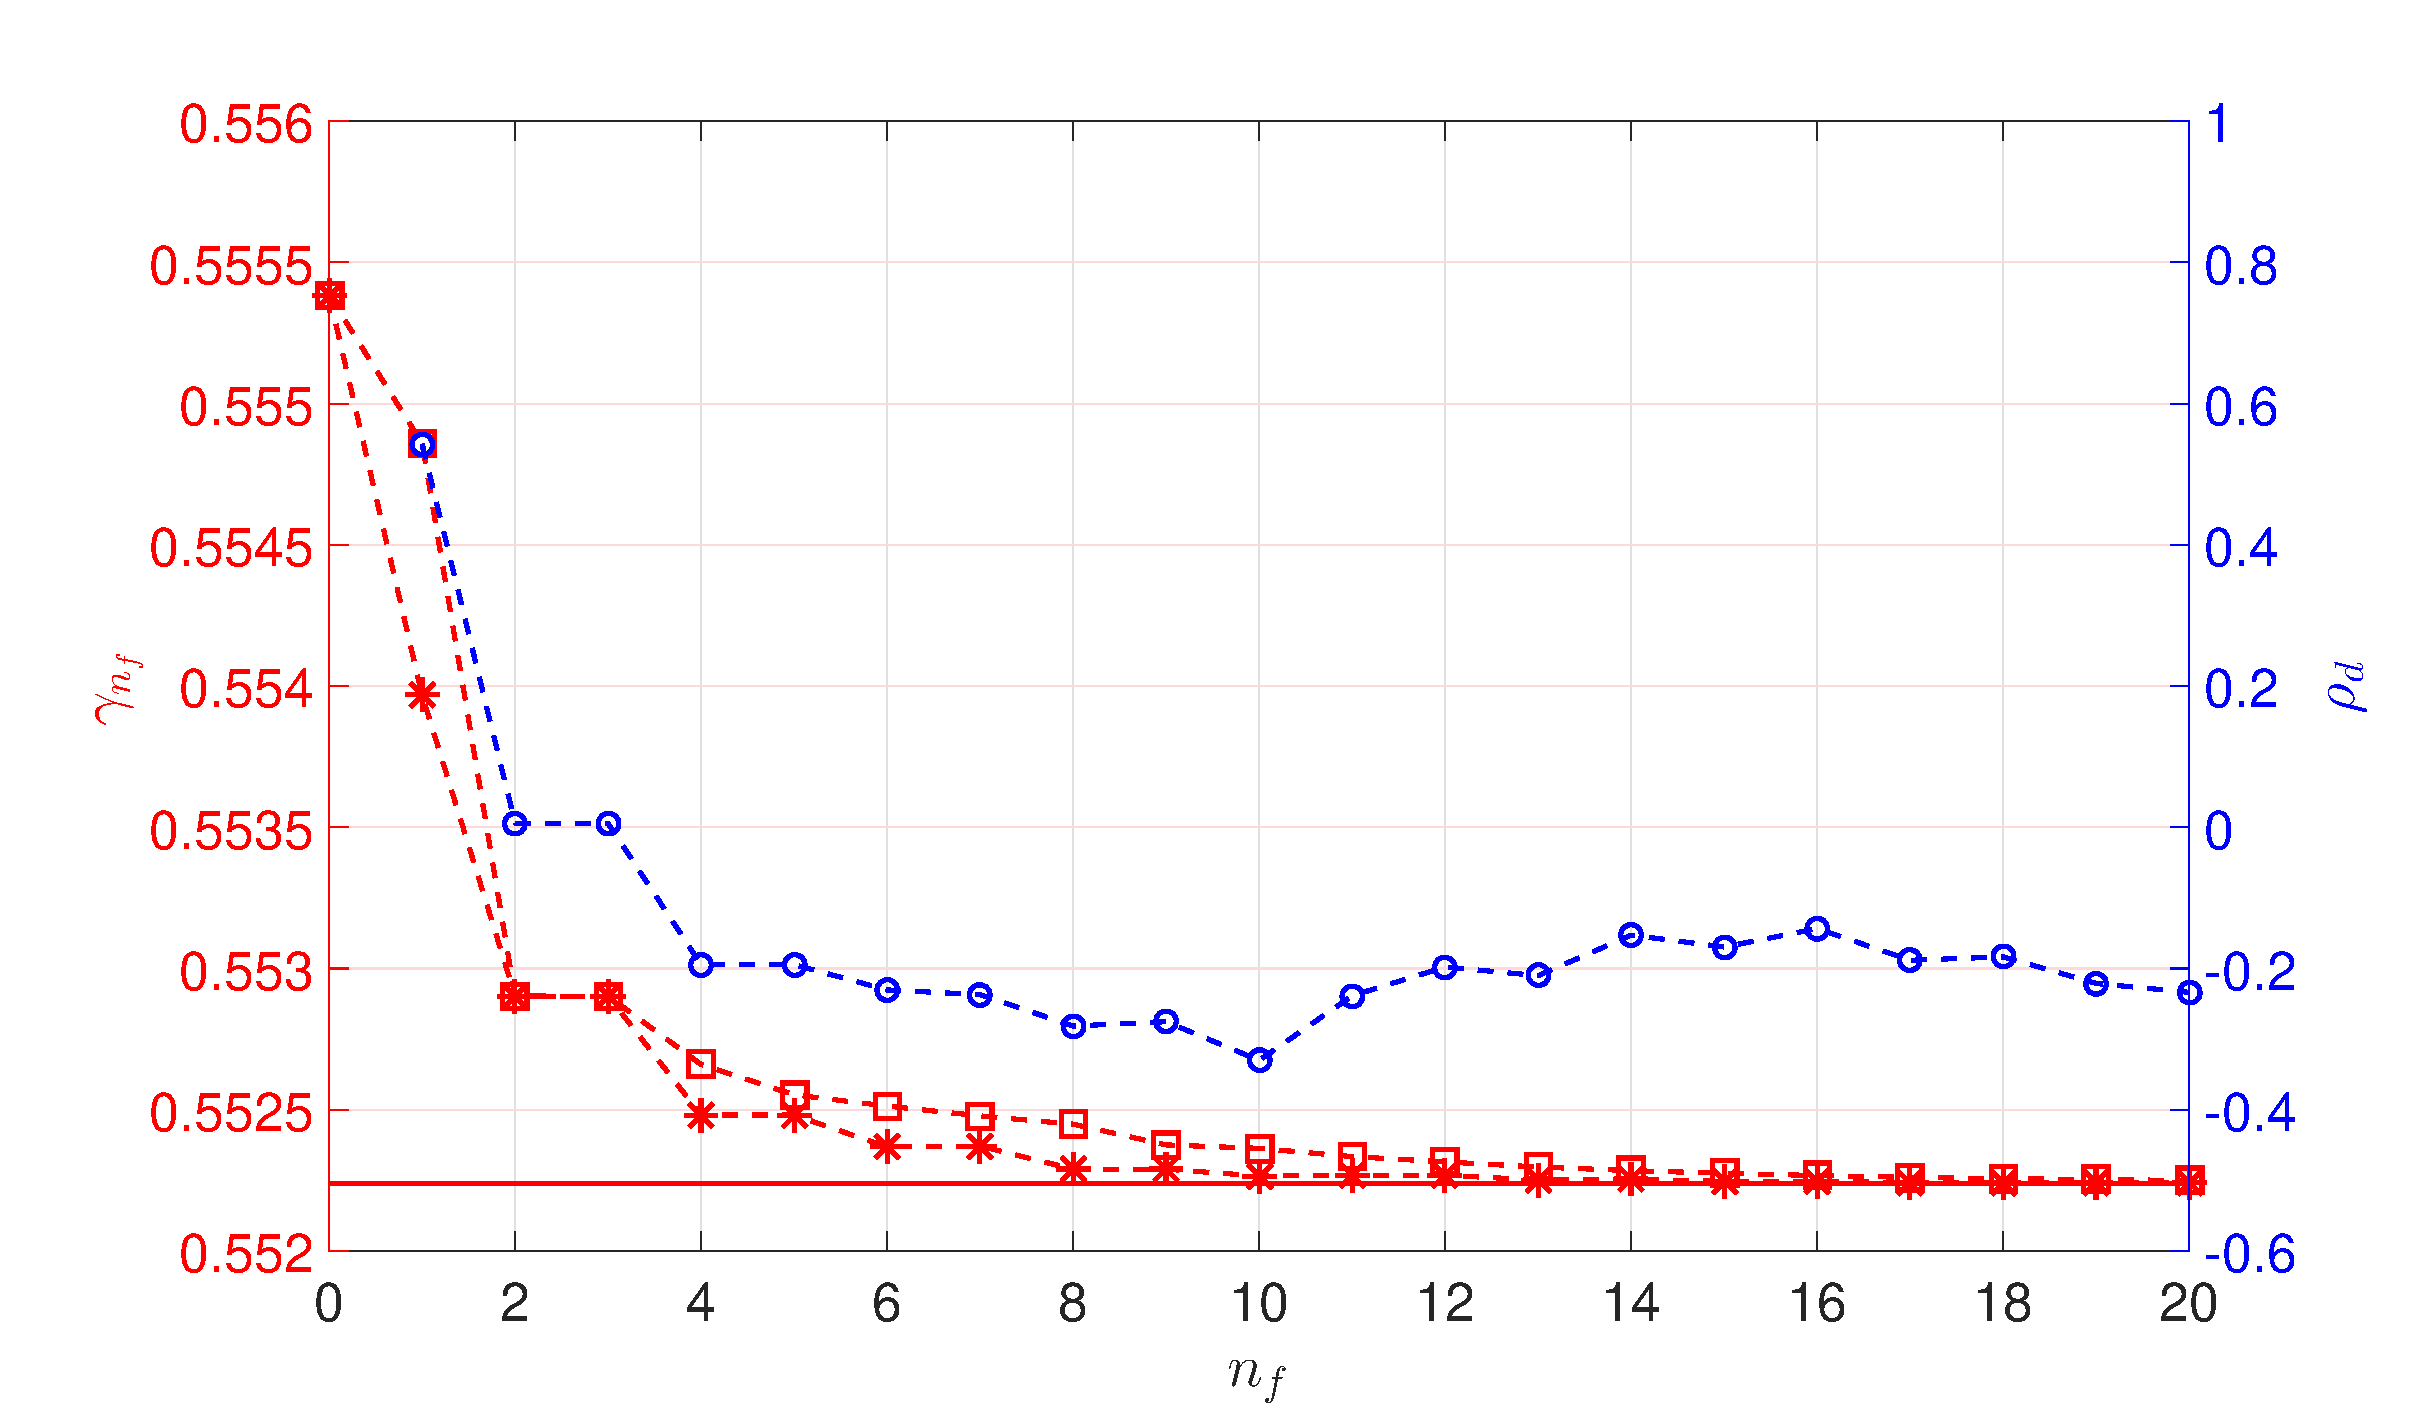
\includegraphics[width=\columnwidth]{../pics/gamma_convergence.eps}
\caption{Optimal solution obtained from \texttt{mixsyn} command (straight-red line); $\gamma_{n_f}$ for $F(\rho)$ as an FIR filter ({\color{red}{- -$\square$- -}});  $\gamma_{n_f}$ for $F(\rho)$ with $\rho_d$ as a decision variable ({\color{red}{- -$*$- -}}); the value of $\rho_d$ when used as a decision variable  ({\color{blue}{- -$\circ$- -}}) }
\label{fig:ex2}
\end{figure}




\subsection{Example 3: Multimodel Uncertainty}
For this example, a robust controller will be designed for a family of unstable systems. This example is taken from the Robust Control Toolbox of \texttt{MATLAB}. The nominal plant model for this family of systems is given as follows:
\begin{equation}
G_0(s) = \frac{2}{s-2}
\end{equation}
This model is perturbed through various types of uncertainties such as time delay, high frequency resonance, pole/gain migration, and extra lag; the family of perturbed models are given as follows:
\begin{equation}
  \begin{split}
    G_1(s) &= G_0(s) \frac{1}{0.06s+1}\\       
    G_2(s) &= G_0(s) \frac{50^2}{s^2+10s+50^2}\\        
    G_3(s) &= G_0(s) \frac{70^2}{s^2+28s+70^2}
  \end{split}
\quad  
  \begin{split}
    G_4(s) &= G_0(s)e^{-0.04s}\\        
    G_5(s) &= \frac{2.4}{s-2.2}\\        
    G_6(s) &= \frac{1.6}{s-1.8}
  \end{split}
\end{equation}
The performance filter $W_1(s)$ and noise filter $W_2(s)$ are chosen to be equal to the filters asserted in \cite{Kar13}, i.e.,:
\begin{equation}
  \begin{split}
    W_1(s) &= \frac{0.33s+4.248}{s+0.008496}\\       
    W_2(s) &= \frac{0.1975s^2+0.6284s+1}{7.901\cdot 10^{-5}s^2+0.2514s+400}
  \end{split}
\end{equation}
For this problem, the control objective is to minimize $\gamma$ and satisfy the following criteria for all seven models:
\begin{equation} \label{eq:mixed_syn}
\|W_1S_{\ell} \|_{\infty} < \gamma \quad \mbox{and} \quad \|W_2T_{\ell} \|_{\infty} < \gamma
\end{equation}
for ${\ell} = 0,\ldots,6$. Note that this control objective satisfies the mixed sensitivity robust condition, and not the robust performance condition in (\ref{eq:inf_norm}). The $\mu$-synthesis approach in the \texttt{MATLAB} Robust Control Toolbox uses this criteria to design a controller. In this approach, a multiplicative uncertainty is considered and an appropriate weighting filter is designed to ensure that the condition in (\ref{eq:mixed_syn}) is satisfied for all seven models. The controller produced by \texttt{MATLAB} with this $\mu$-synthesis approach yields an $18$-th order controller and satisfies the control objective for all models. 

The same problem is now solved using the proposed approach. First, the coprime factors $N_{\ell}(s)$ and $M_{\ell}(s)$ for ${\ell} = 0,\ldots,6$ must be established. Since each model is unstable, then each coprime factor must be selected such that $\{N_{\ell}(s),M_{\ell}(s) \}  \in \mathscr{P}$ for all ${\ell}$. A simple choice is to divide both the numerator and denominator of each model by a factor $(s+\rho_p)^{\lambda_{\ell}}$, where $\rho_p \in \mathbb{R}_+$ and ${\lambda_{\ell}}$ is the largest degree of the denominator of the $\ell$-th respective plant model. For example, the coprime factors for the plant $G_2(s)$ can be formed as follows:
\begin{equation}
N_2(s) = \frac{2 \cdot 50^2 }{(s+\rho_p)^3}, \ M_2(s) = \frac{(s-2)(s^2+10s+50^2) }{(s+\rho_p)^3}
\end{equation}
From these relations, it is evident that $G_2(s) = N_2(s)M_2^{-1}(s)$. To further simplify the design, the same $\rho_p$ can be selected for each $\ell$-th coprime. To solve the convex optimization problem in (\ref{eq:convex_con}), $\rho_p$ must be fixed a priori; however, with the proposed method, $\rho_p$ need not be fixed. 

The optimization problem (with the proposed approach) for the mixed $\mathcal{H}_\infty$ criteria in (\ref{eq:mixed_syn}) can be formulated as follows:
\begin{equation} \label{eq:opt_true_ex3}
\begin{aligned}
& \underset{ \bm{\rho}}{\text{minimize}}
& & \gamma  \\
& \text{subject to:} & & \gamma^{-1} |W_1M_{\ell}(\bm{\rho})Y(\bm{\rho})F(\bm{\rho})| < \Re\{\psi_{\ell}(\bm{\rho}) F(\bm{\rho})\} \\ 
& & &  \gamma^{-1} |W_2N_{\ell}(\bm{\rho})X(\bm{\rho})F(\bm{\rho})| < \Re\{\psi_{\ell}(\bm{\rho}) F(\bm{\rho})\}   \\ 
& & & \omega \in \Omega, \ell = 0,\ldots,6
\end{aligned}
\end{equation}
where $\psi_{\ell} = N_{\ell}(\bm{\rho})X(\bm{\rho}) + M_{\ell}(\bm{\rho})Y(\bm{\rho})$. In solving the above optimization problem, the parameters in $\{\rho_c,\rho_p,\rho_o \}$ will not be fixed, and will be optimized by the nonlinear programming algorithm (as shown with the notation $N_{\ell}(\bm{\rho})$ and $M_{\ell}(\bm{\rho})$). 



\subsubsection{Simulation Results}
The problem in (\ref{eq:opt_true_ex3}) is converted to a SDP problem by considering a logarithmically spaced frequency grid with $Q$ = $200$ points from $\omega_1 = 10^{-3} \: rad/s$ to $\omega_{200} = 10^{4} \: rad/s$. For the convex problem, a $6$-th order controller ($5$-th order controller with one integrator) will be designed by using the Laguerre basis functions defined in (\ref{eq:Laguerre}) with $\rho_c = 20$ and $\rho_p = 100$ (as defined in \cite{KNZ16}). With the proposed method (and for comparative purposes), a $6$-th order controller will also be used while a $20$-th order Laguerre basis function will be considered for $F(\bm{\rho})$ (as defined in (\ref{eq:Laguerre_sum_c})). 

The optimal solutions from several optimization algorithms for satisfying the criteria in (\ref{eq:mixed_syn}) are tabulated in Table.\ref{tab:ex3} (where $n$ is the controller order of the respective method). The table also shows the solutions when the convex optimization problem in \cite{KNZ16} is solved when the variables $\rho_c$ and $\rho_p$ are decision variables (thus making the problem non-convex). It can be observed that the proposed method produces the best performance. 

\begin{table}[]
\centering
\caption{Comparison of optimal solutions}
\label{tab:ex3}
\begin{tabular}{c|c|c|c|c||c}
                                                                              & \begin{tabular}[c]{@{}c@{}} $n$ \end{tabular} & $\rho_c$ & $\rho_p$ & $\rho_o$ & $\gamma$ \\ \hline
\texttt{MATLAB} $\mu$-Synthesis                                               & $18$                                                        & $-$      & $-$      & $-$      & $1.024$  \\ \hline       
                                                                      
\begin{tabular}[c]{@{}c@{}}Algorithm in \cite{KNZ16} \\ (Convex) \end{tabular}   & $6$                                                         & $20$    & $100$     & $-$      & $0.881$  \\ \hline

\begin{tabular}[c]{@{}c@{}}Algorithm in \cite{KNZ16} \\ $\{\rho_p,\rho_c\} \rightarrow$ variable \end{tabular}   & $6$                                                         & $23.89$    & $73.87$     & $-$      & $0.870$  \\ \hline

Proposed method                                                               & $6$                                                         & $16.72$    & $127.1$     & $63.68$     & $0.814$   
\end{tabular}
\end{table}

Figure.~\ref{fig:ex3_1} shows the step response of $S(s)$ (disturbance response) for all seven models using the convex optimization algorithm, while Figure.~\ref{fig:ex3_2} shows the step response of $S(s)$ using the proposed method. It can be observed that the proposed method produces shorter settling times and reduced overshoot. 
\begin{figure}
\centering
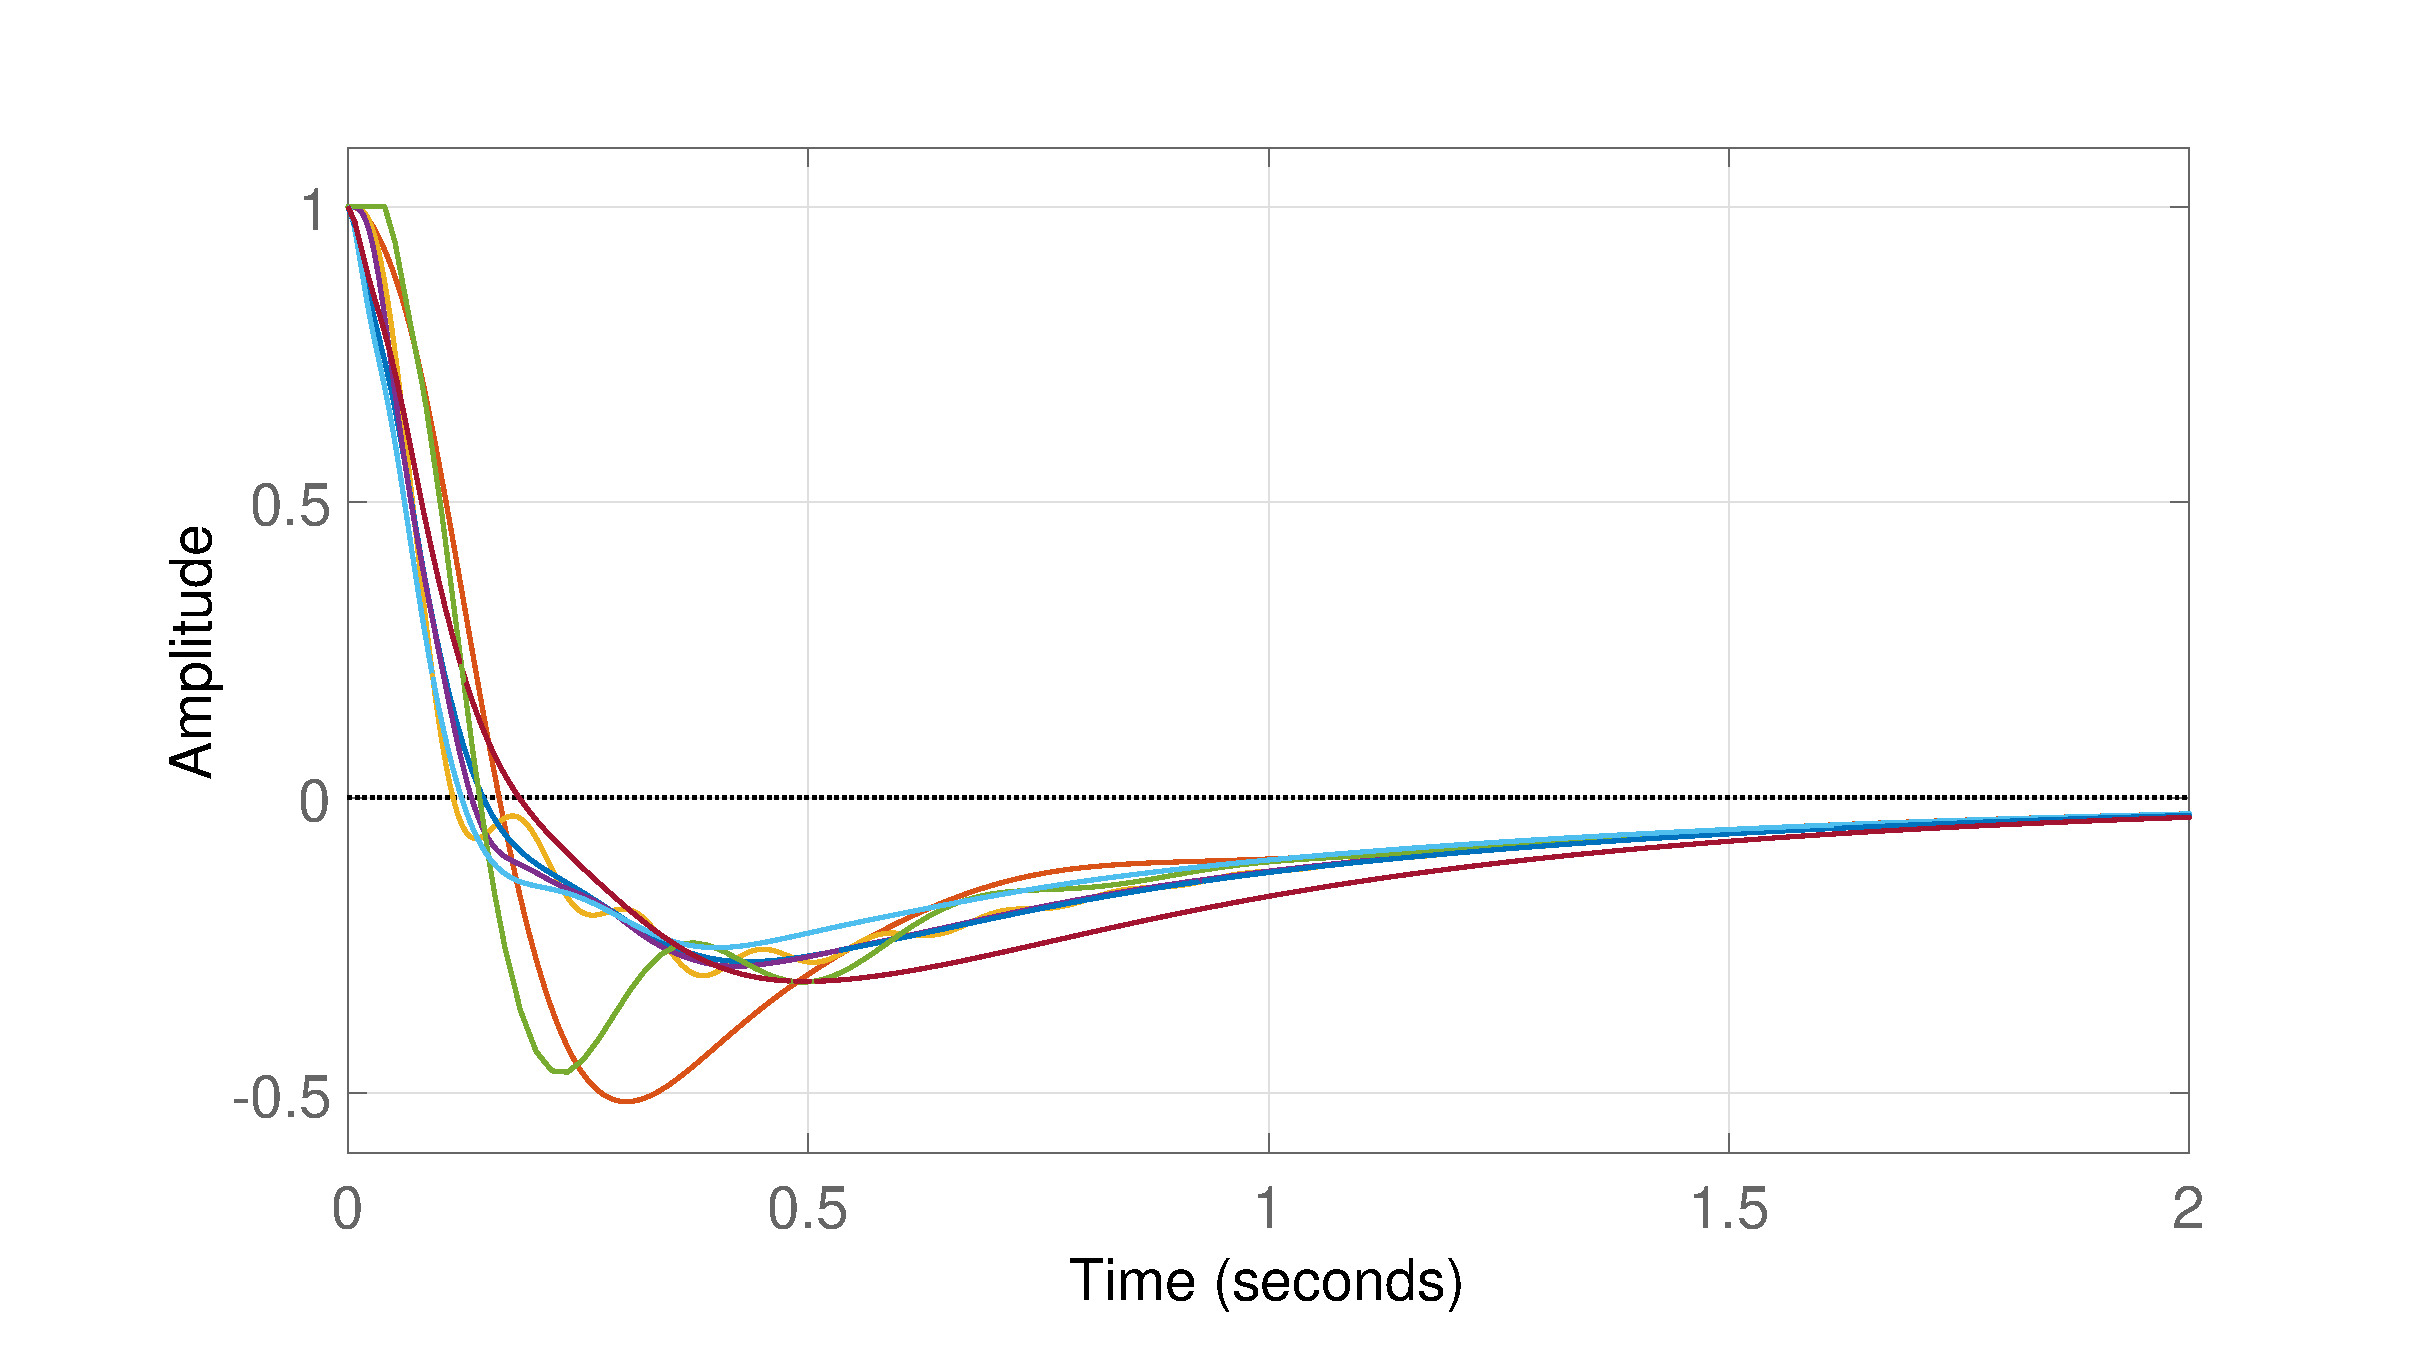
\includegraphics[width=\columnwidth]{../pics/step_multi_convex.eps}
\caption{Step response of $S(s)$ for all seven models using the convex optimization algorithm in \cite{KNZ16}.}
\label{fig:ex3_1}
\end{figure}

\begin{figure}
\centering
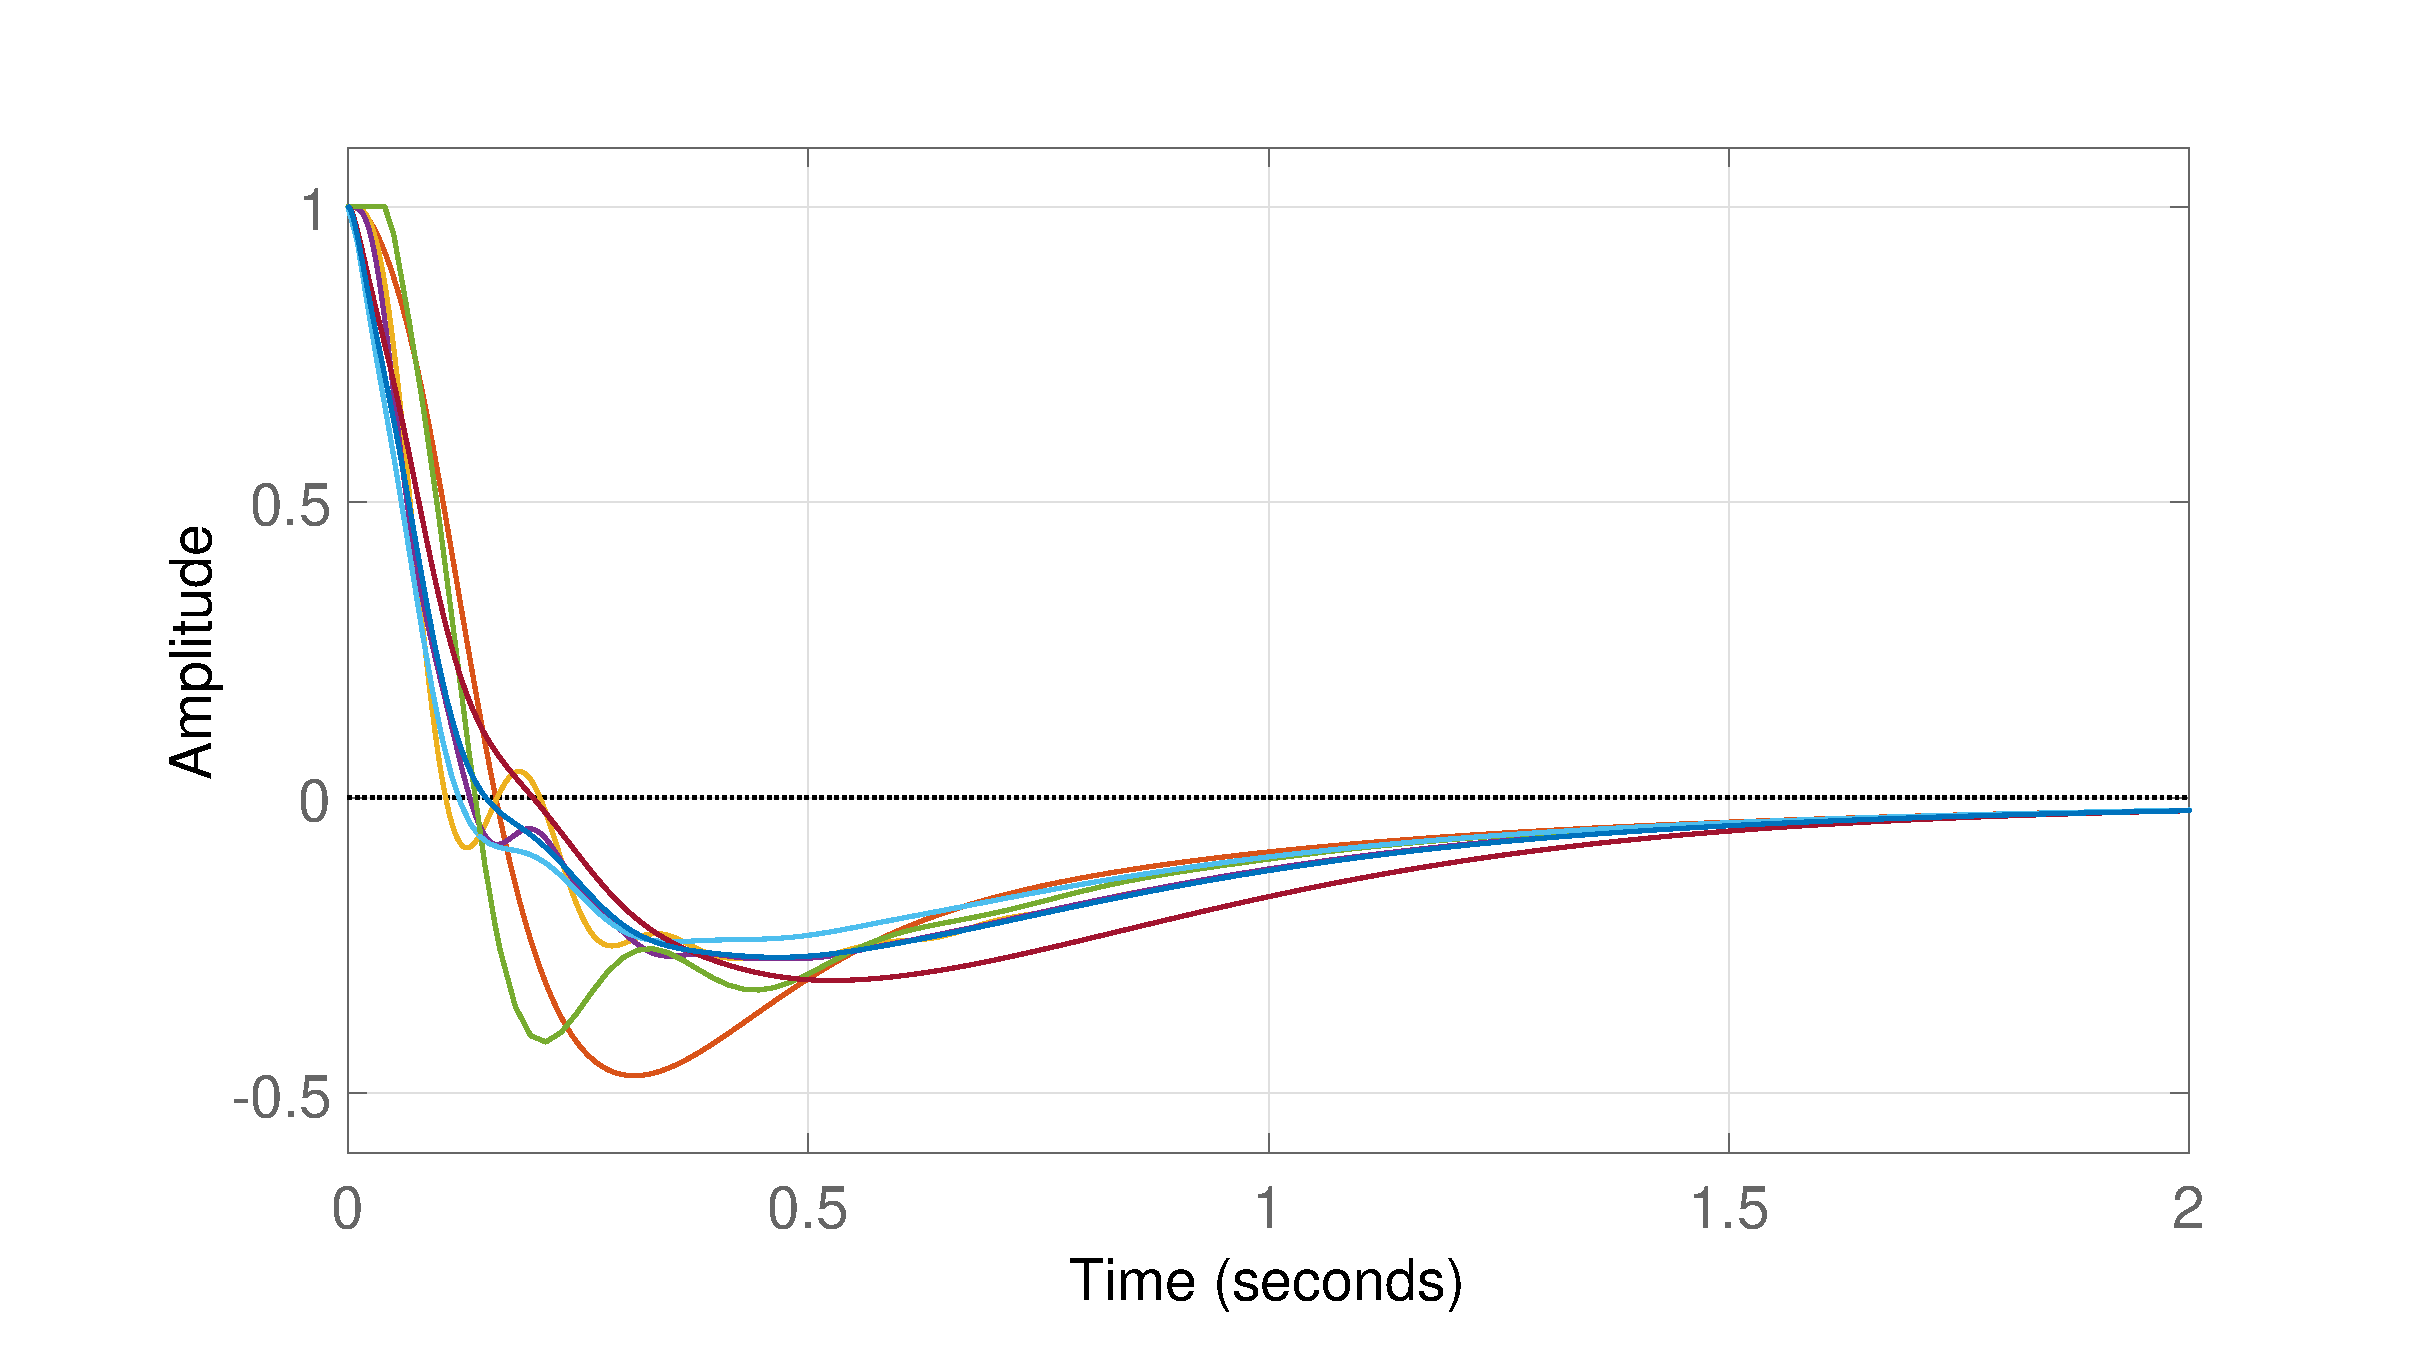
\includegraphics[width=\columnwidth]{../pics/step_multi_optimal.eps}
\caption{Closed-loop step responses with the PID controller parameters asserted in Table.~2 (with $\tau = \tau_n$). Response associated with the proposed PSO algorithm (solid-blue); response associated with the convex optimization algorithm (solid-green); response associated with the robust stability method in \cite{EW09} (solid-red).}
\label{fig:ex3_2}
\end{figure}

\begin{remark*}
The $\mu$-synthesis approach by \texttt{MATLAB} introduces some conservatism in determining the optimal controller. Additionally, with the $\mu$-synthesis approach, the plant $G_4(s)$ was approximated with a first-order Pade function, since pure delay's cannot be used for synthesis. In the proposed approach, the true delay function can be considered in the design while eliminating the conservatism associated with modeling the multi-model uncertainties. 
\end{remark*}


\section{Conclusion} \label{sec:conclusion}
Robust performance can be accomplished by considering the $\mathcal{H}_{\infty}$ control problem. By presetting a frequency grid, an optimization problem can be formulated to minimize the upper-bound of the robust performance condition and solve a finite amount of constraints in the frequency-domain. In this paper, a Non-Death-Penalty approach has been implemented to solve an unconstrained $\mathcal{H}_{\infty}$ problem; the solution to this problem was obtained by realizing a PSO algorithm. From the examples considered in this paper, it is evident that the solutions obtained from the PSO algorithm generate favorable closed-loop responses (with respect to the other methods considered in this paper). In terms of performance, the convex optimization algorithm produces a solution that is comparable to that of the PSO. From the simulation examples, it can be deduced that the solution obtained from the convex optimization algorithm is a good approximation to the solution obtained from the original problem. For further research, it will be desired to investigate how the solution obtained from the PSO algorithm with the $\epsilon$-level comparisons correlates with the solutions obtained in this work.

\bibliography{linear}


\end{document}
